\chapter{Srovnání algoritmů}\label{Srovnání algoritmů}

V této kapitole provedeme srovnání jednotlivých přístupů k řešení hry Snake. Zaměříme se na dvě hlavní kritéria: úspěšnost dokončení hry a efektivitu. Přičemž úspěšností myslíme, jak často algoritmus vede k vítězství - zaplnění celé hrací plochy bez kolize. Efektivitou rozumíme, jak rychle had sbírá jablka a jak plynule se pohybuje bez zbytečných tahů.

Porovnáme tři přístupy na herním poli \(10 \times 10\). Maximální dosažitelné skóre je 97. Prvním je A* (viz Kapitola~\ref{A*}), heuristický algoritmus hledající nejkratší cestu od hlavy hada k jablku. Další je Hamiltonovská kružnice (viz Kapitola~\ref{Hamiltonovská kružnice}), která představuje předem vygenerovanou cestu, jež zajišťuje, že had nikdy nenarazí sám do sebe. Posledním je algorit-\\mus zkratek (viz Kapitola~\ref{Řešení}), který kombinuje Hamiltonovskou kružnici s možností vytvářet optimalizované zkratky pomocí algoritmu A*.

\section{Výsledky A*}

Řešení problému s využitím algoritmu A*, který hledá nejkratší cestu od hlavy hada k jablku, nedopadlo nikdy úspěšně. Had z více než 300 pokusů ani jednou nedohrál hru (nezaplnil celou hrací plochu bez kolize). Průměrná délka hry trvala 21 sekund. Had v průměru dosáhl skóre 28 a průměrný počet tahů byl 223. Na Grafu~\ref{fig:Počet tahů - A_} můžeme vidět četnosti tahů během různých her. Vidíme, že modus počtů tahů je 161-194. V grafu~\ref{fig:Skóre _ Tahy - A_} je znázorněna závislost skóre na počtu tahů. Vidíme, že čím více tahů had udělal, tím většího skóre dosáhl.

\begin{figure}[H]
    \centering
    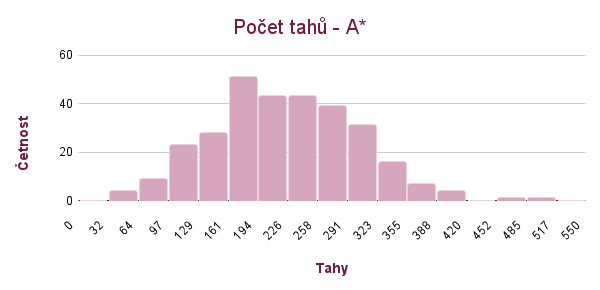
\includegraphics[width=\linewidth]{Images/Počet tahů - A_.png}
    \caption{Četnost tahů během různých her - A*}
    \label{fig:Počet tahů - A_}
\end{figure}

\begin{figure}[H]
    \centering
    \includegraphics[width=\linewidth]{Images/Skóre _ Tahy - A_.png}
    \caption{Závislost skóre na počtu tahů - A*}
    \label{fig:Skóre _ Tahy - A_}
\end{figure}

\section{Hamiltonovská kružnice}

Využití sledování Hamiltonovské kružnice k řešení problému bylo \(100\%\) úspěšné. Průměrná délka hry z 200 pokusů byla 4 minuty a 21 sekund a průměrný počet tahů, který závisí na pozicích generovaných jablek, byl 2485. Největší počet tahů, kterého bylo dosaženo, je 2997 a nejmenší počet tahů byl 1921. V Grafu~\ref{fig:Počet tahů - Hamiltonovská kružnice} je znázorněna četnost tahů během různých her. Je zcela zřejmé, že modus počtů tahů ve hře je 2357-2464.

\begin{figure}[H]
    \centering
    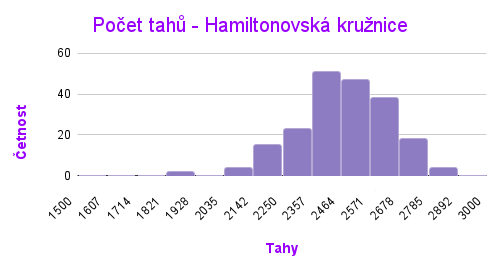
\includegraphics[width=\linewidth]{Images/Počet tahů - Hamiltonovská kružnice.png}
    \caption{Četnost tahů během různých her - Hamiltonovská kružnice}
    \label{fig:Počet tahů - Hamiltonovská kružnice}
\end{figure}

\section{Algoritmus zkratek}

Algoritmus, který vytváří zkratky v existující Hamiltonovské kružnici, vedl v \(72\%\) přípa-\\dech z přibližně 230 pokusů k úspěšnému dokončení hry. V těchto úspěšných pokusech byla průměrná délka hry 3 minuty a 2 sekundy. Průměrný počet tahů, v úspěšných hrách, byl 1825. V Grafu~\ref{fig:Počet tahů - Algoritmus zkratek} je vidět četnost tahů během úspěšných her. Modusy počtů tahů, provedených během hry, jsou 1722-1833 a 1833-1944. Největší počet tahů za jednu hru byl 2112. Tak vysoký počet naznačuje, že had v průběhu hry nevyužil skoro žádné zkratky, protože se počet tahů blíží jednomu z nejmenších počtů tahů, při prostém využití Hamilto-\\novské kružnice. V Grafu~\ref{fig:Tahy _ čas - Algoritmus zkratek} je, z pouze úspěšných pokusů, zobrazena závislost počtu tahů na čase.

\begin{figure}[H]
    \centering
    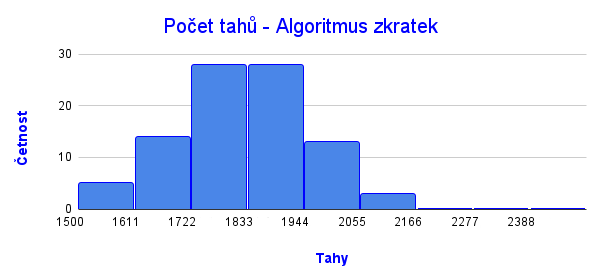
\includegraphics[width=\linewidth]{Images/Počet tahů - Algoritmus zkratek.png}
    \caption{Četnost tahů během různých her - Algoritmus zkratek}
    \label{fig:Počet tahů - Algoritmus zkratek}
\end{figure}

\begin{figure}[H]
    \centering
    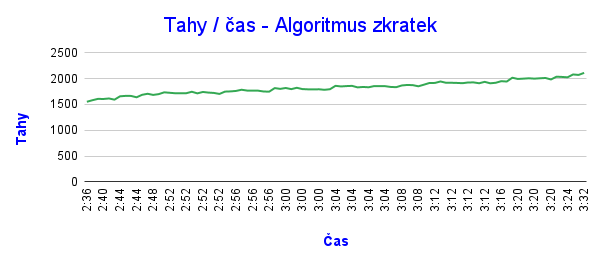
\includegraphics[width=\linewidth]{Images/Tahy _ čas - Algoritmus zkratek.png}
    \caption{Závislost počtu tahů na čase - Algoritmus zkratek}
    \label{fig:Tahy _ čas - Algoritmus zkratek}
\end{figure}

\section{Vzájemné porovnání jednotlivých přístupů}
Pomocí tabulky~\ref{table:PorovnaniPristupu} si porovnáme jednotlivé přístupy. Můžeme vidět, že algoritmus \(A*\), kvůli tomu, že hru nikdy nedokončil, má ve všech měřených oblastech velmi odlišné hodnoty, proto budeme srovnávat spíše algoritmus zkratek a Hamiltonovskou kružnici. Hamiltonovská kružnice byla v dokončení hry \(100\%\) úspěšná, na rozdíl od algoritmu zkratek, který byl úspěšný pouze ze \(72\%\). Průměrná délka úspěšné hry algoritmu zkratek byla 3 minuty a 2 sekundy, což je přibližně o \(30\%\) lepší čas, než u prostého sledování Hamiltonovské kružnice. Průměrný počet tahů, v úspěšných hrách algoritmu zkratek, byl 1825 a to je skoro o 100 tahů méně, než nejmenší počet tahů při využití pouze Hamiltonovské kružnice. Modusy tahů v úspěšných hrách algoritmu zkratek jsou výrazně menší než modus tahů na hru u Hamiltonovské kružnice. 

\begin{table}[h!]
\centering
\begin{tabular}{ | p{4,5cm} || p{1,7cm} | p{2cm} | p{2cm} | p{2cm} |  }
 \hline
 Algoritmus & Úspěšnost v \% & Průměrný čas hry & Průměrný počet tahů na hru & Modus tahů na hru \\
 \hline
 A*  & 0 & 21 s & 223 & 194 \\
 Hamiltonovská kružnice & 100 & 4 min 21 s & 2485 & 2357-2464 \\
 Algoritmus zkratek & 72 & 3 min 2 s & 1825 & 1722-1833, 1833-1944 \\
 \hline
\end{tabular}
\caption{Porovnání jednotlivých přístupů k řešení hry Snake. Porovnáváme úspěšnost dokončení hry, průměrný čas pro dokončení hry, průměrný a nejčetnější počet tahů na hru pro algoritmy A*, Hamiltonovskou kružnici a algoritmus zkratek.}
\label{table:PorovnaniPristupu}
\end{table}

Tato zjištění ukazují, že i když Hamiltonovská kružnice garantuje \(100\%\) úspěšnost, algorit-\\mus zkratek je efektivnější, pokud jde o rychlost dokončení hry a počet tahů. Algoritmus zkratek poskytuje rychlejší a plynulejší hru s nižším počtem tahů, což jej činí nejefektivněj-\\ším přístupem mezi těmito třemi algoritmy pro řešení hry Snake.